\documentclass[twoside]{book}

% Packages required by doxygen
\usepackage{fixltx2e}
\usepackage{calc}
\usepackage{doxygen}
\usepackage[export]{adjustbox} % also loads graphicx
\usepackage{graphicx}
\usepackage[utf8]{inputenc}
\usepackage{makeidx}
\usepackage{multicol}
\usepackage{multirow}
\PassOptionsToPackage{warn}{textcomp}
\usepackage{textcomp}
\usepackage[nointegrals]{wasysym}
\usepackage[table]{xcolor}

% NLS support packages
\usepackage[french]{babel}

% Font selection
\usepackage[T1]{fontenc}
\usepackage[scaled=.90]{helvet}
\usepackage{courier}
\usepackage{amssymb}
\usepackage{sectsty}
\renewcommand{\familydefault}{\sfdefault}
\allsectionsfont{%
  \fontseries{bc}\selectfont%
  \color{darkgray}%
}
\renewcommand{\DoxyLabelFont}{%
  \fontseries{bc}\selectfont%
  \color{darkgray}%
}
\newcommand{\+}{\discretionary{\mbox{\scriptsize$\hookleftarrow$}}{}{}}

% Page & text layout
\usepackage{geometry}
\geometry{%
  a4paper,%
  top=2.5cm,%
  bottom=2.5cm,%
  left=2.5cm,%
  right=2.5cm%
}
\tolerance=750
\hfuzz=15pt
\hbadness=750
\setlength{\emergencystretch}{15pt}
\setlength{\parindent}{0cm}
\setlength{\parskip}{3ex plus 2ex minus 2ex}
\makeatletter
\renewcommand{\paragraph}{%
  \@startsection{paragraph}{4}{0ex}{-1.0ex}{1.0ex}{%
    \normalfont\normalsize\bfseries\SS@parafont%
  }%
}
\renewcommand{\subparagraph}{%
  \@startsection{subparagraph}{5}{0ex}{-1.0ex}{1.0ex}{%
    \normalfont\normalsize\bfseries\SS@subparafont%
  }%
}
\makeatother

% Headers & footers
\usepackage{fancyhdr}
\pagestyle{fancyplain}
\fancyhead[LE]{\fancyplain{}{\bfseries\thepage}}
\fancyhead[CE]{\fancyplain{}{}}
\fancyhead[RE]{\fancyplain{}{\bfseries\leftmark}}
\fancyhead[LO]{\fancyplain{}{\bfseries\rightmark}}
\fancyhead[CO]{\fancyplain{}{}}
\fancyhead[RO]{\fancyplain{}{\bfseries\thepage}}
\fancyfoot[LE]{\fancyplain{}{}}
\fancyfoot[CE]{\fancyplain{}{}}
\fancyfoot[RE]{\fancyplain{}{\bfseries\scriptsize Généré par Doxygen }}
\fancyfoot[LO]{\fancyplain{}{\bfseries\scriptsize Généré par Doxygen }}
\fancyfoot[CO]{\fancyplain{}{}}
\fancyfoot[RO]{\fancyplain{}{}}
\renewcommand{\footrulewidth}{0.4pt}
\renewcommand{\chaptermark}[1]{%
  \markboth{#1}{}%
}
\renewcommand{\sectionmark}[1]{%
  \markright{\thesection\ #1}%
}

% Indices & bibliography
\usepackage{natbib}
\usepackage[titles]{tocloft}
\setcounter{tocdepth}{3}
\setcounter{secnumdepth}{5}
\makeindex

% Hyperlinks (required, but should be loaded last)
\usepackage{ifpdf}
\ifpdf
  \usepackage[pdftex,pagebackref=true]{hyperref}
\else
  \usepackage[ps2pdf,pagebackref=true]{hyperref}
\fi
\hypersetup{%
  colorlinks=true,%
  linkcolor=blue,%
  citecolor=blue,%
  unicode%
}

% Custom commands
\newcommand{\clearemptydoublepage}{%
  \newpage{\pagestyle{empty}\cleardoublepage}%
}

\usepackage{caption}
\captionsetup{labelsep=space,justification=centering,font={bf},singlelinecheck=off,skip=4pt,position=top}

%===== C O N T E N T S =====

\begin{document}

% Titlepage & ToC
\hypersetup{pageanchor=false,
             bookmarksnumbered=true,
             pdfencoding=unicode
            }
\pagenumbering{alph}
\begin{titlepage}
\vspace*{7cm}
\begin{center}%
{\Large Jeu de la Vie \\[1ex]\large 1.\+0 }\\
\vspace*{1cm}
{\large Généré par Doxygen 1.8.13}\\
\end{center}
\end{titlepage}
\clearemptydoublepage
\pagenumbering{roman}
\tableofcontents
\clearemptydoublepage
\pagenumbering{arabic}
\hypersetup{pageanchor=true}

%--- Begin generated contents ---
\chapter{Index des structures de données}
\section{Structures de données}
Liste des structures de données avec une brève description \+:\begin{DoxyCompactList}
\item\contentsline{section}{\hyperlink{structgrille}{grille} }{\pageref{structgrille}}{}
\end{DoxyCompactList}

\chapter{Index des fichiers}
\section{Liste des fichiers}
Liste de tous les fichiers documentés avec une brève description \+:\begin{DoxyCompactList}
\item\contentsline{section}{include/\hyperlink{grille_8h}{grille.\+h} \\*Fichier d\textquotesingle{}en-\/tête du fichier source \hyperlink{grille_8c}{grille.\+c} }{\pageref{grille_8h}}{}
\item\contentsline{section}{include/\hyperlink{io_8h}{io.\+h} \\*Fichier d\textquotesingle{}en-\/tête du fichier source \hyperlink{io_8c}{io.\+c} }{\pageref{io_8h}}{}
\item\contentsline{section}{include/\hyperlink{jeu_8h}{jeu.\+h} \\*Fichier d\textquotesingle{}en-\/tête du fichier source \hyperlink{jeu_8c}{jeu.\+c} }{\pageref{jeu_8h}}{}
\item\contentsline{section}{src/\hyperlink{grille_8c}{grille.\+c} \\*Gestion des grilles du jeu de la vie }{\pageref{grille_8c}}{}
\item\contentsline{section}{src/\hyperlink{io_8c}{io.\+c} \\*Gestion des entrées/sorties du jeu de la vie }{\pageref{io_8c}}{}
\item\contentsline{section}{src/\hyperlink{jeu_8c}{jeu.\+c} \\*Règles du jeu de la vie }{\pageref{jeu_8c}}{}
\item\contentsline{section}{src/\hyperlink{main_8c}{main.\+c} \\*Jeu de la vie }{\pageref{main_8c}}{}
\end{DoxyCompactList}

\chapter{Documentation des structures de données}
\hypertarget{structgrille}{}\section{Référence de la structure grille}
\label{structgrille}\index{grille@{grille}}


{\ttfamily \#include $<$grille.\+h$>$}

\subsection*{Champs de données}
\begin{DoxyCompactItemize}
\item 
\mbox{\Hypertarget{structgrille_acf98b2c5c1a51e021aad6633fd2c41c6}\label{structgrille_acf98b2c5c1a51e021aad6633fd2c41c6}} 
int {\bfseries nbl}
\item 
\mbox{\Hypertarget{structgrille_a965672cdeaba5c5352e804c1ac4bdb91}\label{structgrille_a965672cdeaba5c5352e804c1ac4bdb91}} 
int {\bfseries nbc}
\item 
\mbox{\Hypertarget{structgrille_a008dfdfef8fc75a738819f5329ee57a7}\label{structgrille_a008dfdfef8fc75a738819f5329ee57a7}} 
int $\ast$$\ast$ {\bfseries cellules}
\end{DoxyCompactItemize}


\subsection{Description détaillée}
Une grille est définie par un nombre de lignes, un nombre de colonnes et un tableau de tableaux de cellules. 

La documentation de cette structure a été générée à partir du fichier suivant \+:\begin{DoxyCompactItemize}
\item 
include/\hyperlink{grille_8h}{grille.\+h}\end{DoxyCompactItemize}

\chapter{Documentation des fichiers}
\hypertarget{grille_8h}{}\section{Référence du fichier include/grille.h}
\label{grille_8h}\index{include/grille.\+h@{include/grille.\+h}}


Fichier d\textquotesingle{}en-\/tête du fichier source \hyperlink{grille_8c}{grille.\+c}.  


{\ttfamily \#include $<$stdlib.\+h$>$}\newline
{\ttfamily \#include $<$stdio.\+h$>$}\newline
{\ttfamily \#include $<$assert.\+h$>$}\newline
Graphe des dépendances par inclusion de grille.\+h\+:\nopagebreak
\begin{figure}[H]
\begin{center}
\leavevmode
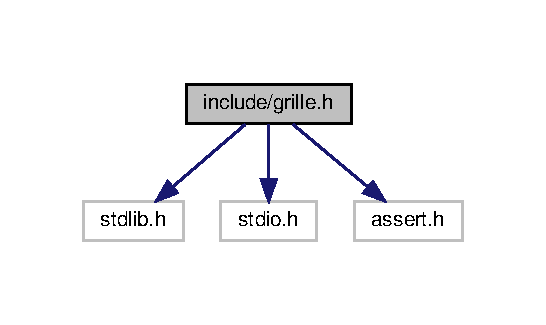
\includegraphics[width=262pt]{grille_8h__incl}
\end{center}
\end{figure}
Ce graphe montre quels fichiers incluent directement ou indirectement ce fichier \+:\nopagebreak
\begin{figure}[H]
\begin{center}
\leavevmode
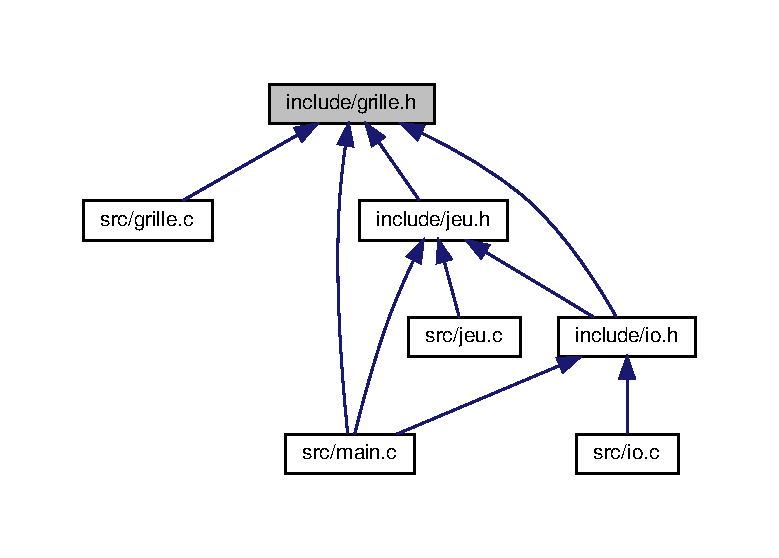
\includegraphics[width=350pt]{grille_8h__dep__incl}
\end{center}
\end{figure}
\subsection*{Structures de données}
\begin{DoxyCompactItemize}
\item 
struct \hyperlink{structgrille}{grille}
\end{DoxyCompactItemize}
\subsection*{Fonctions}
\begin{DoxyCompactItemize}
\item 
void \hyperlink{grille_8h_ae621f51c60aa4fafaa0c9f6c9b5a4036}{alloue\+\_\+grille} (int l, int c, \hyperlink{structgrille}{grille} $\ast$g)
\begin{DoxyCompactList}\small\item\em Fonction d\textquotesingle{}allocation d\textquotesingle{}une grille de taille l$\ast$c, initialise toutes les cellules à mortes. \end{DoxyCompactList}\item 
void \hyperlink{grille_8h_a7074b2b15576e9d2b3cd15c3a1dc7012}{libere\+\_\+grille} (\hyperlink{structgrille}{grille} $\ast$g)
\begin{DoxyCompactList}\small\item\em Fonction de libération d\textquotesingle{}une grille. \end{DoxyCompactList}\item 
void \hyperlink{grille_8h_adf5501cc0bbad28f5ffc561d92197e4e}{init\+\_\+grille\+\_\+from\+\_\+file} (char $\ast$filename, \hyperlink{structgrille}{grille} $\ast$g)
\begin{DoxyCompactList}\small\item\em Fonction d\textquotesingle{}allocation et d\textquotesingle{}initalisation d\textquotesingle{}une grille à partir d\textquotesingle{}un fichier. \end{DoxyCompactList}\item 
static void \hyperlink{grille_8h_a889ff6b0976dfb79007387ad30d9c790}{set\+\_\+vivante} (int i, int j, \hyperlink{structgrille}{grille} g)
\begin{DoxyCompactList}\small\item\em Fonction rendant vivante la cellule \mbox{[}i,j\mbox{]} d\textquotesingle{}une grille. \end{DoxyCompactList}\item 
static void \hyperlink{grille_8h_ab5ab346bdf3a9d7e3a0bfeab40416d6e}{set\+\_\+morte} (int i, int j, \hyperlink{structgrille}{grille} g)
\begin{DoxyCompactList}\small\item\em Fonction rendant morte la cellule \mbox{[}i,j\mbox{]} d\textquotesingle{}une grille. \end{DoxyCompactList}\item 
static int \hyperlink{grille_8h_a4a27d70711027eca191df5592f922001}{est\+\_\+vivante} (int i, int j, \hyperlink{structgrille}{grille} g)
\begin{DoxyCompactList}\small\item\em Fonction testant si la cellule \mbox{[}i,j\mbox{]} d\textquotesingle{}une grille est vivante. \end{DoxyCompactList}\item 
void \hyperlink{grille_8h_a63b3ae16c86b568f6aa8f9ce84128b1e}{copie\+\_\+grille} (\hyperlink{structgrille}{grille} gs, \hyperlink{structgrille}{grille} gd)
\begin{DoxyCompactList}\small\item\em Fonction de copie d\textquotesingle{}une grille (sans allocation). \end{DoxyCompactList}\end{DoxyCompactItemize}


\subsection{Description détaillée}
Fichier d\textquotesingle{}en-\/tête du fichier source \hyperlink{grille_8c}{grille.\+c}. 

\begin{DoxyAuthor}{Auteur}
Massimo Venuti 
\end{DoxyAuthor}


\subsection{Documentation des fonctions}
\mbox{\Hypertarget{grille_8h_ae621f51c60aa4fafaa0c9f6c9b5a4036}\label{grille_8h_ae621f51c60aa4fafaa0c9f6c9b5a4036}} 
\index{grille.\+h@{grille.\+h}!alloue\+\_\+grille@{alloue\+\_\+grille}}
\index{alloue\+\_\+grille@{alloue\+\_\+grille}!grille.\+h@{grille.\+h}}
\subsubsection{\texorpdfstring{alloue\+\_\+grille()}{alloue\_grille()}}
{\footnotesize\ttfamily void alloue\+\_\+grille (\begin{DoxyParamCaption}\item[{int}]{l,  }\item[{int}]{c,  }\item[{\hyperlink{structgrille}{grille} $\ast$}]{g }\end{DoxyParamCaption})}



Fonction d\textquotesingle{}allocation d\textquotesingle{}une grille de taille l$\ast$c, initialise toutes les cellules à mortes. 


\begin{DoxyParams}{Paramètres}
{\em l} & Entier \+: nombre de lignes. \\
\hline
{\em c} & Entier \+: nombre de colonnes. \\
\hline
{\em g} & Adresse de la grille à allouer. \\
\hline
\end{DoxyParams}
\mbox{\Hypertarget{grille_8h_a63b3ae16c86b568f6aa8f9ce84128b1e}\label{grille_8h_a63b3ae16c86b568f6aa8f9ce84128b1e}} 
\index{grille.\+h@{grille.\+h}!copie\+\_\+grille@{copie\+\_\+grille}}
\index{copie\+\_\+grille@{copie\+\_\+grille}!grille.\+h@{grille.\+h}}
\subsubsection{\texorpdfstring{copie\+\_\+grille()}{copie\_grille()}}
{\footnotesize\ttfamily void copie\+\_\+grille (\begin{DoxyParamCaption}\item[{\hyperlink{structgrille}{grille}}]{gs,  }\item[{\hyperlink{structgrille}{grille}}]{gd }\end{DoxyParamCaption})}



Fonction de copie d\textquotesingle{}une grille (sans allocation). 


\begin{DoxyParams}{Paramètres}
{\em gs} & Grille \+: grille à copier (source). \\
\hline
{\em gd} & Grille \+: grille à modifier (destination). \\
\hline
\end{DoxyParams}
\mbox{\Hypertarget{grille_8h_a4a27d70711027eca191df5592f922001}\label{grille_8h_a4a27d70711027eca191df5592f922001}} 
\index{grille.\+h@{grille.\+h}!est\+\_\+vivante@{est\+\_\+vivante}}
\index{est\+\_\+vivante@{est\+\_\+vivante}!grille.\+h@{grille.\+h}}
\subsubsection{\texorpdfstring{est\+\_\+vivante()}{est\_vivante()}}
{\footnotesize\ttfamily static inline int est\+\_\+vivante (\begin{DoxyParamCaption}\item[{int}]{i,  }\item[{int}]{j,  }\item[{\hyperlink{structgrille}{grille}}]{g }\end{DoxyParamCaption})\hspace{0.3cm}{\ttfamily [inline]}, {\ttfamily [static]}}



Fonction testant si la cellule \mbox{[}i,j\mbox{]} d\textquotesingle{}une grille est vivante. 


\begin{DoxyParams}{Paramètres}
{\em i} & Entier \+: i-\/ème ligne de la grille. \\
\hline
{\em j} & Entier \+: j-\/ème ligne de la grille \\
\hline
{\em g} & Grille \+: grille en jeu. \\
\hline
\end{DoxyParams}
\mbox{\Hypertarget{grille_8h_adf5501cc0bbad28f5ffc561d92197e4e}\label{grille_8h_adf5501cc0bbad28f5ffc561d92197e4e}} 
\index{grille.\+h@{grille.\+h}!init\+\_\+grille\+\_\+from\+\_\+file@{init\+\_\+grille\+\_\+from\+\_\+file}}
\index{init\+\_\+grille\+\_\+from\+\_\+file@{init\+\_\+grille\+\_\+from\+\_\+file}!grille.\+h@{grille.\+h}}
\subsubsection{\texorpdfstring{init\+\_\+grille\+\_\+from\+\_\+file()}{init\_grille\_from\_file()}}
{\footnotesize\ttfamily void init\+\_\+grille\+\_\+from\+\_\+file (\begin{DoxyParamCaption}\item[{char $\ast$}]{filename,  }\item[{\hyperlink{structgrille}{grille} $\ast$}]{g }\end{DoxyParamCaption})}



Fonction d\textquotesingle{}allocation et d\textquotesingle{}initalisation d\textquotesingle{}une grille à partir d\textquotesingle{}un fichier. 


\begin{DoxyParams}{Paramètres}
{\em filename} & Chaine de caractères \+: nom du fichier dans lequel se trouve la configuration initiale de la grille. \\
\hline
{\em g} & Adresse de la grille à initialiser. \\
\hline
\end{DoxyParams}
\mbox{\Hypertarget{grille_8h_a7074b2b15576e9d2b3cd15c3a1dc7012}\label{grille_8h_a7074b2b15576e9d2b3cd15c3a1dc7012}} 
\index{grille.\+h@{grille.\+h}!libere\+\_\+grille@{libere\+\_\+grille}}
\index{libere\+\_\+grille@{libere\+\_\+grille}!grille.\+h@{grille.\+h}}
\subsubsection{\texorpdfstring{libere\+\_\+grille()}{libere\_grille()}}
{\footnotesize\ttfamily void libere\+\_\+grille (\begin{DoxyParamCaption}\item[{\hyperlink{structgrille}{grille} $\ast$}]{g }\end{DoxyParamCaption})}



Fonction de libération d\textquotesingle{}une grille. 


\begin{DoxyParams}{Paramètres}
{\em g} & Adresse de la grille à libérer. \\
\hline
\end{DoxyParams}
\mbox{\Hypertarget{grille_8h_ab5ab346bdf3a9d7e3a0bfeab40416d6e}\label{grille_8h_ab5ab346bdf3a9d7e3a0bfeab40416d6e}} 
\index{grille.\+h@{grille.\+h}!set\+\_\+morte@{set\+\_\+morte}}
\index{set\+\_\+morte@{set\+\_\+morte}!grille.\+h@{grille.\+h}}
\subsubsection{\texorpdfstring{set\+\_\+morte()}{set\_morte()}}
{\footnotesize\ttfamily static inline void set\+\_\+morte (\begin{DoxyParamCaption}\item[{int}]{i,  }\item[{int}]{j,  }\item[{\hyperlink{structgrille}{grille}}]{g }\end{DoxyParamCaption})\hspace{0.3cm}{\ttfamily [inline]}, {\ttfamily [static]}}



Fonction rendant morte la cellule \mbox{[}i,j\mbox{]} d\textquotesingle{}une grille. 


\begin{DoxyParams}{Paramètres}
{\em i} & Entier \+: i-\/ème ligne de la grille. \\
\hline
{\em j} & Entier \+: j-\/ème ligne de la grille \\
\hline
{\em g} & Grille \+: grille en jeu. \\
\hline
\end{DoxyParams}
\mbox{\Hypertarget{grille_8h_a889ff6b0976dfb79007387ad30d9c790}\label{grille_8h_a889ff6b0976dfb79007387ad30d9c790}} 
\index{grille.\+h@{grille.\+h}!set\+\_\+vivante@{set\+\_\+vivante}}
\index{set\+\_\+vivante@{set\+\_\+vivante}!grille.\+h@{grille.\+h}}
\subsubsection{\texorpdfstring{set\+\_\+vivante()}{set\_vivante()}}
{\footnotesize\ttfamily static inline void set\+\_\+vivante (\begin{DoxyParamCaption}\item[{int}]{i,  }\item[{int}]{j,  }\item[{\hyperlink{structgrille}{grille}}]{g }\end{DoxyParamCaption})\hspace{0.3cm}{\ttfamily [inline]}, {\ttfamily [static]}}



Fonction rendant vivante la cellule \mbox{[}i,j\mbox{]} d\textquotesingle{}une grille. 


\begin{DoxyParams}{Paramètres}
{\em i} & Entier \+: i-\/ème ligne de la grille. \\
\hline
{\em j} & Entier \+: j-\/ème ligne de la grille \\
\hline
{\em g} & Grille \+: grille en jeu. \\
\hline
\end{DoxyParams}

\hypertarget{io_8h}{}\section{Référence du fichier include/io.h}
\label{io_8h}\index{include/io.\+h@{include/io.\+h}}


Fichier d\textquotesingle{}en-\/tête du fichier source \hyperlink{io_8c}{io.\+c}.  


{\ttfamily \#include $<$stdio.\+h$>$}\newline
{\ttfamily \#include $<$string.\+h$>$}\newline
{\ttfamily \#include \char`\"{}grille.\+h\char`\"{}}\newline
{\ttfamily \#include \char`\"{}jeu.\+h\char`\"{}}\newline
Graphe des dépendances par inclusion de io.\+h\+:
\nopagebreak
\begin{figure}[H]
\begin{center}
\leavevmode
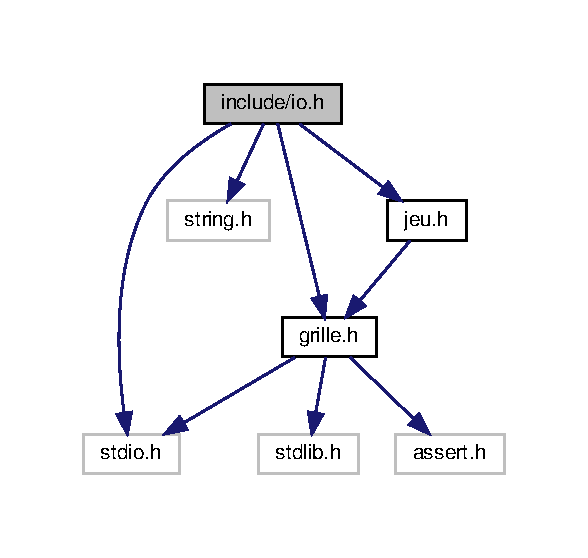
\includegraphics[width=282pt]{io_8h__incl}
\end{center}
\end{figure}
Ce graphe montre quels fichiers incluent directement ou indirectement ce fichier \+:
\nopagebreak
\begin{figure}[H]
\begin{center}
\leavevmode
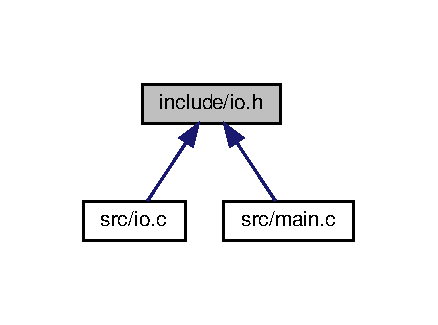
\includegraphics[width=210pt]{io_8h__dep__incl}
\end{center}
\end{figure}
\subsection*{Macros}
\begin{DoxyCompactItemize}
\item 
\mbox{\Hypertarget{io_8h_ae6ad0540d5109a0200f0dde5dc5b4bf6}\label{io_8h_ae6ad0540d5109a0200f0dde5dc5b4bf6}} 
\#define {\bfseries T\+A\+I\+L\+L\+E\+\_\+\+M\+AX}~200
\item 
\mbox{\Hypertarget{io_8h_a9098362cc46e6d6c6d6ed065ec4261a8}\label{io_8h_a9098362cc46e6d6c6d6ed065ec4261a8}} 
\#define {\bfseries P\+E\+R\+I\+O\+D\+E\+\_\+\+I\+N\+IT}~-\/1
\end{DoxyCompactItemize}
\subsection*{Fonctions}
\begin{DoxyCompactItemize}
\item 
void \hyperlink{io_8h_a634cf584c380ce221d5d4199f3e813bd}{affiche\+\_\+trait} (int c)
\begin{DoxyCompactList}\small\item\em Fonction d\textquotesingle{}affichage d\textquotesingle{}un trait horizontal en mode Texte. \end{DoxyCompactList}\item 
void \hyperlink{io_8h_a3f3ff78e56fcf21a932ff73b70635554}{affiche\+\_\+ligne} (int c, int $\ast$ligne)
\begin{DoxyCompactList}\small\item\em Fonction d\textquotesingle{}affichage d\textquotesingle{}une ligne de la grille en mode Texte. \end{DoxyCompactList}\item 
void \hyperlink{io_8h_a90cb8ec05374b46d9995705ed4954f34}{affiche\+\_\+grille} (\hyperlink{structgrille}{grille} g)
\begin{DoxyCompactList}\small\item\em Fonction d\textquotesingle{}affichage d\textquotesingle{}une grille en mode Texte. \end{DoxyCompactList}\item 
void \hyperlink{io_8h_ab36a6f8957cd3e682119007836ce6ad5}{efface\+\_\+grille} (\hyperlink{structgrille}{grille} g)
\begin{DoxyCompactList}\small\item\em Fonction d\textquotesingle{}effacement d\textquotesingle{}une grille en mode Texte. \end{DoxyCompactList}\item 
void \hyperlink{io_8h_a88493b3c55828670e47150a95ed7db5b}{debut\+\_\+jeu} (\hyperlink{structgrille}{grille} $\ast$g, \hyperlink{structgrille}{grille} $\ast$gc)
\begin{DoxyCompactList}\small\item\em Fonction pour débuter le jeu en mode Texte. \end{DoxyCompactList}\item 
void \hyperlink{io_8h_afec97c7f0ca09173b533e29ff31bd286}{affiche\+\_\+temps} (int temps)
\begin{DoxyCompactList}\small\item\em Fonction d\textquotesingle{}affichage du temps d\textquotesingle{}évolution courant en mode Texte. \end{DoxyCompactList}\item 
void \hyperlink{io_8h_a92cca3b39e4f5e70fac85ea3d96690a5}{affiche\+\_\+oscillation} (int periode)
\begin{DoxyCompactList}\small\item\em Fonction d\textquotesingle{}affichage de la période d\textquotesingle{}évolution d\textquotesingle{}une grille en mode Texte. \end{DoxyCompactList}\item 
\mbox{\Hypertarget{io_8h_a0811ccbaa0cf73f604b98cd760adbc91}\label{io_8h_a0811ccbaa0cf73f604b98cd760adbc91}} 
void \hyperlink{io_8h_a0811ccbaa0cf73f604b98cd760adbc91}{affiche\+\_\+vieillissement} ()
\begin{DoxyCompactList}\small\item\em Fonction d\textquotesingle{}affichage de l\textquotesingle{}état du vieillissement (O\+N/\+O\+FF) en mode Texte. \end{DoxyCompactList}\item 
\mbox{\Hypertarget{io_8h_aa49ae01960af6777be7df4da33fff6fc}\label{io_8h_aa49ae01960af6777be7df4da33fff6fc}} 
void \hyperlink{io_8h_aa49ae01960af6777be7df4da33fff6fc}{affiche\+\_\+calcul\+\_\+voisinage} ()
\begin{DoxyCompactList}\small\item\em Fonction d\textquotesingle{}affichage de l\textquotesingle{}état du voisinage cyclique (O\+N/\+O\+FF) en mode Texte. \end{DoxyCompactList}\item 
\mbox{\Hypertarget{io_8h_a352250d421c748fcda925bd74a390361}\label{io_8h_a352250d421c748fcda925bd74a390361}} 
void {\bfseries affichage} (\hyperlink{structgrille}{grille} $\ast$g, int temps, int periode)
\end{DoxyCompactItemize}
\subsection*{Variables}
\begin{DoxyCompactItemize}
\item 
\mbox{\Hypertarget{io_8h_af587b56ea61a80b468caff5a89715cd7}\label{io_8h_af587b56ea61a80b468caff5a89715cd7}} 
int($\ast$ \hyperlink{io_8h_af587b56ea61a80b468caff5a89715cd7}{compte\+\_\+voisins\+\_\+vivants} )(int, int, \hyperlink{structgrille}{grille})
\begin{DoxyCompactList}\small\item\em Pointeur de fonction contenant l\textquotesingle{}adresse de la fonction de calcul du voisinage d\textquotesingle{}une cellule. \end{DoxyCompactList}\item 
\mbox{\Hypertarget{io_8h_a852233e3ec97f7c44944c67998337e26}\label{io_8h_a852233e3ec97f7c44944c67998337e26}} 
int \hyperlink{io_8h_a852233e3ec97f7c44944c67998337e26}{vieillissement}
\begin{DoxyCompactList}\small\item\em Valeur contenant 1 ou 0 selon si le vieillissement des cellules est activé ou non. \end{DoxyCompactList}\end{DoxyCompactItemize}


\subsection{Description détaillée}
Fichier d\textquotesingle{}en-\/tête du fichier source \hyperlink{io_8c}{io.\+c}. 

\begin{DoxyAuthor}{Auteur}
Massimo Venuti 
\end{DoxyAuthor}


\subsection{Documentation des fonctions}
\mbox{\Hypertarget{io_8h_a90cb8ec05374b46d9995705ed4954f34}\label{io_8h_a90cb8ec05374b46d9995705ed4954f34}} 
\index{io.\+h@{io.\+h}!affiche\+\_\+grille@{affiche\+\_\+grille}}
\index{affiche\+\_\+grille@{affiche\+\_\+grille}!io.\+h@{io.\+h}}
\subsubsection{\texorpdfstring{affiche\+\_\+grille()}{affiche\_grille()}}
{\footnotesize\ttfamily void affiche\+\_\+grille (\begin{DoxyParamCaption}\item[{\hyperlink{structgrille}{grille}}]{g }\end{DoxyParamCaption})}



Fonction d\textquotesingle{}affichage d\textquotesingle{}une grille en mode Texte. 


\begin{DoxyParams}{Paramètres}
{\em g} & Grille \+: grille à afficher. \\
\hline
\end{DoxyParams}
\mbox{\Hypertarget{io_8h_a3f3ff78e56fcf21a932ff73b70635554}\label{io_8h_a3f3ff78e56fcf21a932ff73b70635554}} 
\index{io.\+h@{io.\+h}!affiche\+\_\+ligne@{affiche\+\_\+ligne}}
\index{affiche\+\_\+ligne@{affiche\+\_\+ligne}!io.\+h@{io.\+h}}
\subsubsection{\texorpdfstring{affiche\+\_\+ligne()}{affiche\_ligne()}}
{\footnotesize\ttfamily void affiche\+\_\+ligne (\begin{DoxyParamCaption}\item[{int}]{c,  }\item[{int $\ast$}]{ligne }\end{DoxyParamCaption})}



Fonction d\textquotesingle{}affichage d\textquotesingle{}une ligne de la grille en mode Texte. 


\begin{DoxyParams}{Paramètres}
{\em c} & Entier \+: nombre de colonnes de la grille. \\
\hline
{\em ligne} & Tableau d\textquotesingle{}entiers \+: ligne de la grille. \\
\hline
\end{DoxyParams}
\mbox{\Hypertarget{io_8h_a92cca3b39e4f5e70fac85ea3d96690a5}\label{io_8h_a92cca3b39e4f5e70fac85ea3d96690a5}} 
\index{io.\+h@{io.\+h}!affiche\+\_\+oscillation@{affiche\+\_\+oscillation}}
\index{affiche\+\_\+oscillation@{affiche\+\_\+oscillation}!io.\+h@{io.\+h}}
\subsubsection{\texorpdfstring{affiche\+\_\+oscillation()}{affiche\_oscillation()}}
{\footnotesize\ttfamily void affiche\+\_\+oscillation (\begin{DoxyParamCaption}\item[{int}]{periode }\end{DoxyParamCaption})}



Fonction d\textquotesingle{}affichage de la période d\textquotesingle{}évolution d\textquotesingle{}une grille en mode Texte. 


\begin{DoxyParams}{Paramètres}
{\em periode} & Entier \+: période d\textquotesingle{}oscillation de la grille courante. \\
\hline
\end{DoxyParams}
\mbox{\Hypertarget{io_8h_afec97c7f0ca09173b533e29ff31bd286}\label{io_8h_afec97c7f0ca09173b533e29ff31bd286}} 
\index{io.\+h@{io.\+h}!affiche\+\_\+temps@{affiche\+\_\+temps}}
\index{affiche\+\_\+temps@{affiche\+\_\+temps}!io.\+h@{io.\+h}}
\subsubsection{\texorpdfstring{affiche\+\_\+temps()}{affiche\_temps()}}
{\footnotesize\ttfamily void affiche\+\_\+temps (\begin{DoxyParamCaption}\item[{int}]{temps }\end{DoxyParamCaption})}



Fonction d\textquotesingle{}affichage du temps d\textquotesingle{}évolution courant en mode Texte. 


\begin{DoxyParams}{Paramètres}
{\em temps} & Entier \+: temps d\textquotesingle{}évolution courant. \\
\hline
\end{DoxyParams}
\mbox{\Hypertarget{io_8h_a634cf584c380ce221d5d4199f3e813bd}\label{io_8h_a634cf584c380ce221d5d4199f3e813bd}} 
\index{io.\+h@{io.\+h}!affiche\+\_\+trait@{affiche\+\_\+trait}}
\index{affiche\+\_\+trait@{affiche\+\_\+trait}!io.\+h@{io.\+h}}
\subsubsection{\texorpdfstring{affiche\+\_\+trait()}{affiche\_trait()}}
{\footnotesize\ttfamily void affiche\+\_\+trait (\begin{DoxyParamCaption}\item[{int}]{c }\end{DoxyParamCaption})}



Fonction d\textquotesingle{}affichage d\textquotesingle{}un trait horizontal en mode Texte. 


\begin{DoxyParams}{Paramètres}
{\em c} & Entier \+: nombre de colonnes de la grille. \\
\hline
\end{DoxyParams}
\mbox{\Hypertarget{io_8h_a88493b3c55828670e47150a95ed7db5b}\label{io_8h_a88493b3c55828670e47150a95ed7db5b}} 
\index{io.\+h@{io.\+h}!debut\+\_\+jeu@{debut\+\_\+jeu}}
\index{debut\+\_\+jeu@{debut\+\_\+jeu}!io.\+h@{io.\+h}}
\subsubsection{\texorpdfstring{debut\+\_\+jeu()}{debut\_jeu()}}
{\footnotesize\ttfamily void debut\+\_\+jeu (\begin{DoxyParamCaption}\item[{\hyperlink{structgrille}{grille} $\ast$}]{g,  }\item[{\hyperlink{structgrille}{grille} $\ast$}]{gc }\end{DoxyParamCaption})}



Fonction pour débuter le jeu en mode Texte. 


\begin{DoxyParams}{Paramètres}
{\em gc} & Adresse de la grille servant de copie temporaire pour le programme. \\
\hline
{\em g} & Adresse de la grille en jeu. \\
\hline
\end{DoxyParams}
\mbox{\Hypertarget{io_8h_ab36a6f8957cd3e682119007836ce6ad5}\label{io_8h_ab36a6f8957cd3e682119007836ce6ad5}} 
\index{io.\+h@{io.\+h}!efface\+\_\+grille@{efface\+\_\+grille}}
\index{efface\+\_\+grille@{efface\+\_\+grille}!io.\+h@{io.\+h}}
\subsubsection{\texorpdfstring{efface\+\_\+grille()}{efface\_grille()}}
{\footnotesize\ttfamily void efface\+\_\+grille (\begin{DoxyParamCaption}\item[{\hyperlink{structgrille}{grille}}]{g }\end{DoxyParamCaption})}



Fonction d\textquotesingle{}effacement d\textquotesingle{}une grille en mode Texte. 


\begin{DoxyParams}{Paramètres}
{\em g} & Grille \+: grille à effacer. \\
\hline
\end{DoxyParams}

\hypertarget{jeu_8h}{}\section{Référence du fichier include/jeu.h}
\label{jeu_8h}\index{include/jeu.\+h@{include/jeu.\+h}}


Fichier d\textquotesingle{}en-\/tête du fichier source \hyperlink{jeu_8c}{jeu.\+c}.  


{\ttfamily \#include \char`\"{}grille.\+h\char`\"{}}\newline
Graphe des dépendances par inclusion de jeu.\+h\+:
\nopagebreak
\begin{figure}[H]
\begin{center}
\leavevmode
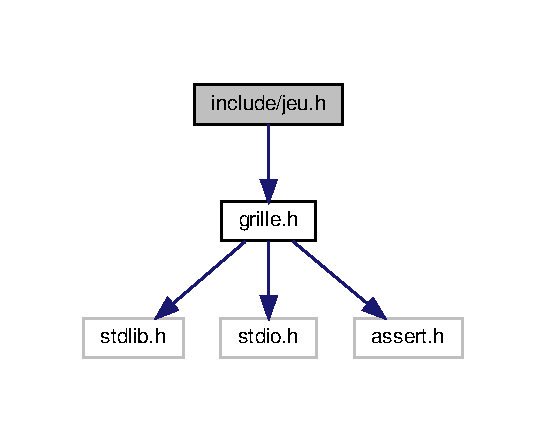
\includegraphics[width=262pt]{jeu_8h__incl}
\end{center}
\end{figure}
Ce graphe montre quels fichiers incluent directement ou indirectement ce fichier \+:
\nopagebreak
\begin{figure}[H]
\begin{center}
\leavevmode
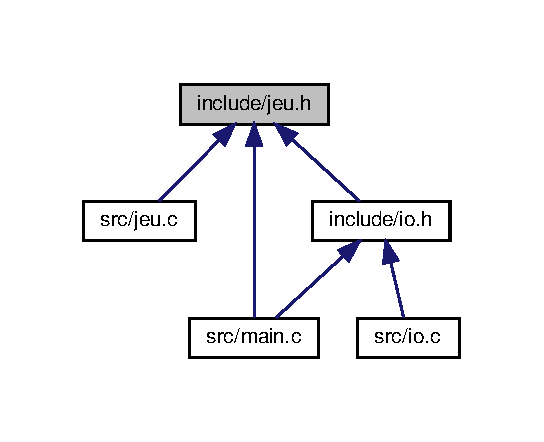
\includegraphics[width=350pt]{jeu_8h__dep__incl}
\end{center}
\end{figure}
\subsection*{Macros}
\begin{DoxyCompactItemize}
\item 
\mbox{\Hypertarget{jeu_8h_a711cc76b16996b0312dfa1f24f183f3c}\label{jeu_8h_a711cc76b16996b0312dfa1f24f183f3c}} 
\#define {\bfseries V\+I\+E\+I\+L\+L\+I\+S\+S\+E\+M\+E\+N\+T\+\_\+\+I\+N\+IT}~1
\item 
\mbox{\Hypertarget{jeu_8h_a6cdb10a572da681b1f293759439f437e}\label{jeu_8h_a6cdb10a572da681b1f293759439f437e}} 
\#define {\bfseries T\+E\+M\+P\+S\+\_\+\+I\+N\+IT}~1
\item 
\mbox{\Hypertarget{jeu_8h_a625e382d1726d52b7fd65f723f0532ca}\label{jeu_8h_a625e382d1726d52b7fd65f723f0532ca}} 
\#define {\bfseries P\+E\+R\+I\+O\+D\+E\+\_\+\+M\+AX}~50
\end{DoxyCompactItemize}
\subsection*{Fonctions}
\begin{DoxyCompactItemize}
\item 
static int \hyperlink{jeu_8h_a8cc2b5e88ad337fae1efad3f36d33f01}{modulo} (int i, int m)
\begin{DoxyCompactList}\small\item\em Fonction modulo modifiée. \end{DoxyCompactList}\item 
int \hyperlink{jeu_8h_a919a35926d94b71717909ecc50233f26}{compte\+\_\+voisins\+\_\+vivants\+\_\+cyclique} (int i, int j, \hyperlink{structgrille}{grille} g)
\begin{DoxyCompactList}\small\item\em Fonction renvoyant le nombre de voisins vivants d\textquotesingle{}une cellule \mbox{[}i,j\mbox{]} -\/ les bords sont cycliques. \end{DoxyCompactList}\item 
int \hyperlink{jeu_8h_a2e8fdd206d197391527920bbbc137eef}{compte\+\_\+voisins\+\_\+vivants\+\_\+non\+\_\+cyclique} (int i, int j, \hyperlink{structgrille}{grille} g)
\begin{DoxyCompactList}\small\item\em Fonction renvoyant le nombre de voisins vivants d\textquotesingle{}une cellule \mbox{[}i,j\mbox{]} -\/ les bords ne sont pas cycliques. \end{DoxyCompactList}\item 
\mbox{\Hypertarget{jeu_8h_a35492cdc239f17e2ef5fd447c11db14a}\label{jeu_8h_a35492cdc239f17e2ef5fd447c11db14a}} 
void \hyperlink{jeu_8h_a35492cdc239f17e2ef5fd447c11db14a}{toggle\+\_\+compte\+\_\+voisins\+\_\+vivants} ()
\begin{DoxyCompactList}\small\item\em Fonction activant/désactivant le mode cyclique. \end{DoxyCompactList}\item 
\mbox{\Hypertarget{jeu_8h_af5dc5f87c713e0c76ead7327db4518f0}\label{jeu_8h_af5dc5f87c713e0c76ead7327db4518f0}} 
void \hyperlink{jeu_8h_af5dc5f87c713e0c76ead7327db4518f0}{toggle\+\_\+vieillissement} ()
\begin{DoxyCompactList}\small\item\em Fonction activant/désactivant le vieillissement. \end{DoxyCompactList}\item 
int \hyperlink{jeu_8h_a97d70fd6528087d6d64f63510f62b65d}{periode\+\_\+oscillation\+\_\+courante} (\hyperlink{structgrille}{grille} g)
\begin{DoxyCompactList}\small\item\em Fonction renvoyant la période d\textquotesingle{}oscillation d\textquotesingle{}une grille dans son état courant. \end{DoxyCompactList}\item 
int \hyperlink{jeu_8h_aba0c5411f74b76f13ccb2eac63175753}{periode\+\_\+oscillation\+\_\+delai} (\hyperlink{structgrille}{grille} g)
\begin{DoxyCompactList}\small\item\em Fonction renvoyant la période d\textquotesingle{}oscillation d\textquotesingle{}une grille en considérant un éventuel délai. \end{DoxyCompactList}\item 
void \hyperlink{jeu_8h_ada8f751a97ad1847db23c5ba17be7802}{evolue} (\hyperlink{structgrille}{grille} $\ast$g, \hyperlink{structgrille}{grille} $\ast$gc)
\begin{DoxyCompactList}\small\item\em Fonction faisant évoluer une grille d\textquotesingle{}un pas de temps. \end{DoxyCompactList}\end{DoxyCompactItemize}


\subsection{Description détaillée}
Fichier d\textquotesingle{}en-\/tête du fichier source \hyperlink{jeu_8c}{jeu.\+c}. 

\begin{DoxyAuthor}{Auteur}
Massimo Venuti 
\end{DoxyAuthor}


\subsection{Documentation des fonctions}
\mbox{\Hypertarget{jeu_8h_a919a35926d94b71717909ecc50233f26}\label{jeu_8h_a919a35926d94b71717909ecc50233f26}} 
\index{jeu.\+h@{jeu.\+h}!compte\+\_\+voisins\+\_\+vivants\+\_\+cyclique@{compte\+\_\+voisins\+\_\+vivants\+\_\+cyclique}}
\index{compte\+\_\+voisins\+\_\+vivants\+\_\+cyclique@{compte\+\_\+voisins\+\_\+vivants\+\_\+cyclique}!jeu.\+h@{jeu.\+h}}
\subsubsection{\texorpdfstring{compte\+\_\+voisins\+\_\+vivants\+\_\+cyclique()}{compte\_voisins\_vivants\_cyclique()}}
{\footnotesize\ttfamily int compte\+\_\+voisins\+\_\+vivants\+\_\+cyclique (\begin{DoxyParamCaption}\item[{int}]{i,  }\item[{int}]{j,  }\item[{\hyperlink{structgrille}{grille}}]{g }\end{DoxyParamCaption})}



Fonction renvoyant le nombre de voisins vivants d\textquotesingle{}une cellule \mbox{[}i,j\mbox{]} -\/ les bords sont cycliques. 


\begin{DoxyParams}{Paramètres}
{\em i} & Entier \+: i-\/ème ligne de la grille. \\
\hline
{\em j} & Entier \+: j-\/ème colonne de la grille. \\
\hline
{\em g} & Grille \+: grille en jeu. \\
\hline
\end{DoxyParams}
\begin{DoxyReturn}{Renvoie}
Entier \+: nombre de voisins vivants de la cellule. 
\end{DoxyReturn}
\mbox{\Hypertarget{jeu_8h_a2e8fdd206d197391527920bbbc137eef}\label{jeu_8h_a2e8fdd206d197391527920bbbc137eef}} 
\index{jeu.\+h@{jeu.\+h}!compte\+\_\+voisins\+\_\+vivants\+\_\+non\+\_\+cyclique@{compte\+\_\+voisins\+\_\+vivants\+\_\+non\+\_\+cyclique}}
\index{compte\+\_\+voisins\+\_\+vivants\+\_\+non\+\_\+cyclique@{compte\+\_\+voisins\+\_\+vivants\+\_\+non\+\_\+cyclique}!jeu.\+h@{jeu.\+h}}
\subsubsection{\texorpdfstring{compte\+\_\+voisins\+\_\+vivants\+\_\+non\+\_\+cyclique()}{compte\_voisins\_vivants\_non\_cyclique()}}
{\footnotesize\ttfamily int compte\+\_\+voisins\+\_\+vivants\+\_\+non\+\_\+cyclique (\begin{DoxyParamCaption}\item[{int}]{i,  }\item[{int}]{j,  }\item[{\hyperlink{structgrille}{grille}}]{g }\end{DoxyParamCaption})}



Fonction renvoyant le nombre de voisins vivants d\textquotesingle{}une cellule \mbox{[}i,j\mbox{]} -\/ les bords ne sont pas cycliques. 


\begin{DoxyParams}{Paramètres}
{\em i} & Entier \+: i-\/ème ligne de la grille. \\
\hline
{\em j} & Entier \+: j-\/ème colonne de la grille. \\
\hline
{\em g} & Grille \+: grille en jeu. \\
\hline
\end{DoxyParams}
\begin{DoxyReturn}{Renvoie}
Entier \+: nombre de voisins vivants de la cellule. 
\end{DoxyReturn}
\mbox{\Hypertarget{jeu_8h_ada8f751a97ad1847db23c5ba17be7802}\label{jeu_8h_ada8f751a97ad1847db23c5ba17be7802}} 
\index{jeu.\+h@{jeu.\+h}!evolue@{evolue}}
\index{evolue@{evolue}!jeu.\+h@{jeu.\+h}}
\subsubsection{\texorpdfstring{evolue()}{evolue()}}
{\footnotesize\ttfamily void evolue (\begin{DoxyParamCaption}\item[{\hyperlink{structgrille}{grille} $\ast$}]{g,  }\item[{\hyperlink{structgrille}{grille} $\ast$}]{gc }\end{DoxyParamCaption})}



Fonction faisant évoluer une grille d\textquotesingle{}un pas de temps. 


\begin{DoxyParams}{Paramètres}
{\em gc} & Adresse de la grille servant de copie temporaire pour le programme. \\
\hline
{\em g} & Adresse de la grille en jeu. \\
\hline
\end{DoxyParams}
\mbox{\Hypertarget{jeu_8h_a8cc2b5e88ad337fae1efad3f36d33f01}\label{jeu_8h_a8cc2b5e88ad337fae1efad3f36d33f01}} 
\index{jeu.\+h@{jeu.\+h}!modulo@{modulo}}
\index{modulo@{modulo}!jeu.\+h@{jeu.\+h}}
\subsubsection{\texorpdfstring{modulo()}{modulo()}}
{\footnotesize\ttfamily static inline int modulo (\begin{DoxyParamCaption}\item[{int}]{i,  }\item[{int}]{m }\end{DoxyParamCaption})\hspace{0.3cm}{\ttfamily [inline]}, {\ttfamily [static]}}



Fonction modulo modifiée. 


\begin{DoxyParams}{Paramètres}
{\em i} & Entier \+: premier opérande. \\
\hline
{\em m} & Entier \+: second opérande. \\
\hline
\end{DoxyParams}
\begin{DoxyReturn}{Renvoie}
Entier \+: résultat du modulo modifié (i+m)m. 
\end{DoxyReturn}
\mbox{\Hypertarget{jeu_8h_a97d70fd6528087d6d64f63510f62b65d}\label{jeu_8h_a97d70fd6528087d6d64f63510f62b65d}} 
\index{jeu.\+h@{jeu.\+h}!periode\+\_\+oscillation\+\_\+courante@{periode\+\_\+oscillation\+\_\+courante}}
\index{periode\+\_\+oscillation\+\_\+courante@{periode\+\_\+oscillation\+\_\+courante}!jeu.\+h@{jeu.\+h}}
\subsubsection{\texorpdfstring{periode\+\_\+oscillation\+\_\+courante()}{periode\_oscillation\_courante()}}
{\footnotesize\ttfamily int periode\+\_\+oscillation\+\_\+courante (\begin{DoxyParamCaption}\item[{\hyperlink{structgrille}{grille}}]{g }\end{DoxyParamCaption})}



Fonction renvoyant la période d\textquotesingle{}oscillation d\textquotesingle{}une grille dans son état courant. 


\begin{DoxyParams}{Paramètres}
{\em g} & Grille \+: grille en jeu. \\
\hline
\end{DoxyParams}
\begin{DoxyReturn}{Renvoie}
Entier \+: période d\textquotesingle{}oscillation, 0 si elle n\textquotesingle{}existe pas. 
\end{DoxyReturn}
\mbox{\Hypertarget{jeu_8h_aba0c5411f74b76f13ccb2eac63175753}\label{jeu_8h_aba0c5411f74b76f13ccb2eac63175753}} 
\index{jeu.\+h@{jeu.\+h}!periode\+\_\+oscillation\+\_\+delai@{periode\+\_\+oscillation\+\_\+delai}}
\index{periode\+\_\+oscillation\+\_\+delai@{periode\+\_\+oscillation\+\_\+delai}!jeu.\+h@{jeu.\+h}}
\subsubsection{\texorpdfstring{periode\+\_\+oscillation\+\_\+delai()}{periode\_oscillation\_delai()}}
{\footnotesize\ttfamily int periode\+\_\+oscillation\+\_\+delai (\begin{DoxyParamCaption}\item[{\hyperlink{structgrille}{grille}}]{g }\end{DoxyParamCaption})}



Fonction renvoyant la période d\textquotesingle{}oscillation d\textquotesingle{}une grille en considérant un éventuel délai. 


\begin{DoxyParams}{Paramètres}
{\em g} & Grille \+: grille en jeu. \\
\hline
\end{DoxyParams}
\begin{DoxyReturn}{Renvoie}
Entier \+: période d\textquotesingle{}oscillation, 0 si elle n\textquotesingle{}existe pas. 
\end{DoxyReturn}

\hypertarget{grille_8c}{}\section{Référence du fichier src/grille.c}
\label{grille_8c}\index{src/grille.\+c@{src/grille.\+c}}


Gestion des grilles du jeu de la vie.  


{\ttfamily \#include \char`\"{}grille.\+h\char`\"{}}\newline
Graphe des dépendances par inclusion de grille.\+c\+:\nopagebreak
\begin{figure}[H]
\begin{center}
\leavevmode
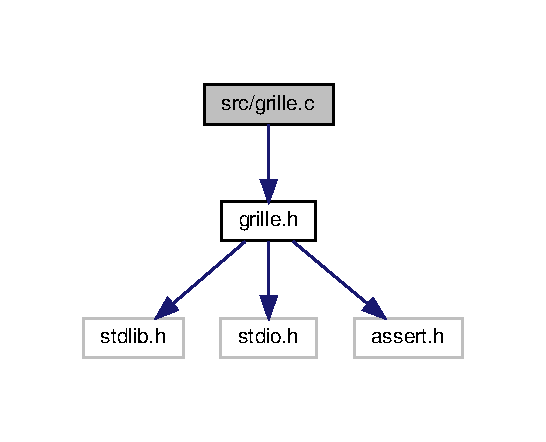
\includegraphics[width=262pt]{grille_8c__incl}
\end{center}
\end{figure}
\subsection*{Fonctions}
\begin{DoxyCompactItemize}
\item 
void \hyperlink{grille_8c_ae621f51c60aa4fafaa0c9f6c9b5a4036}{alloue\+\_\+grille} (int l, int c, \hyperlink{structgrille}{grille} $\ast$g)
\begin{DoxyCompactList}\small\item\em Fonction d\textquotesingle{}allocation d\textquotesingle{}une grille de taille l$\ast$c, initialise toutes les cellules à mortes. \end{DoxyCompactList}\item 
void \hyperlink{grille_8c_a7074b2b15576e9d2b3cd15c3a1dc7012}{libere\+\_\+grille} (\hyperlink{structgrille}{grille} $\ast$g)
\begin{DoxyCompactList}\small\item\em Fonction de libération d\textquotesingle{}une grille. \end{DoxyCompactList}\item 
void \hyperlink{grille_8c_adf5501cc0bbad28f5ffc561d92197e4e}{init\+\_\+grille\+\_\+from\+\_\+file} (char $\ast$filename, \hyperlink{structgrille}{grille} $\ast$g)
\begin{DoxyCompactList}\small\item\em Fonction d\textquotesingle{}allocation et d\textquotesingle{}initalisation d\textquotesingle{}une grille à partir d\textquotesingle{}un fichier. \end{DoxyCompactList}\item 
void \hyperlink{grille_8c_a63b3ae16c86b568f6aa8f9ce84128b1e}{copie\+\_\+grille} (\hyperlink{structgrille}{grille} gs, \hyperlink{structgrille}{grille} gd)
\begin{DoxyCompactList}\small\item\em Fonction de copie d\textquotesingle{}une grille -\/ sans allocation. \end{DoxyCompactList}\item 
int \hyperlink{grille_8c_a043efcb92192aae5f06fcde249370d3c}{sont\+\_\+identiques} (\hyperlink{structgrille}{grille} g1, \hyperlink{structgrille}{grille} g2)
\begin{DoxyCompactList}\small\item\em Fonction comparant 2 grilles -\/ les âges des cellules ne sont pas considérés. \end{DoxyCompactList}\item 
int \hyperlink{grille_8c_a2d61b8d9bac6516500c0157ad4d57c85}{grille\+\_\+vide} (\hyperlink{structgrille}{grille} g)
\begin{DoxyCompactList}\small\item\em Fonction vérifiant si une grille est vide. \end{DoxyCompactList}\end{DoxyCompactItemize}


\subsection{Description détaillée}
Gestion des grilles du jeu de la vie. 

\begin{DoxyAuthor}{Auteur}
Massimo Venuti
\end{DoxyAuthor}
Création / destruction et accès aux fichiers externes des grilles du jeu de la vie. 

\subsection{Documentation des fonctions}
\mbox{\Hypertarget{grille_8c_ae621f51c60aa4fafaa0c9f6c9b5a4036}\label{grille_8c_ae621f51c60aa4fafaa0c9f6c9b5a4036}} 
\index{grille.\+c@{grille.\+c}!alloue\+\_\+grille@{alloue\+\_\+grille}}
\index{alloue\+\_\+grille@{alloue\+\_\+grille}!grille.\+c@{grille.\+c}}
\subsubsection{\texorpdfstring{alloue\+\_\+grille()}{alloue\_grille()}}
{\footnotesize\ttfamily void alloue\+\_\+grille (\begin{DoxyParamCaption}\item[{int}]{l,  }\item[{int}]{c,  }\item[{\hyperlink{structgrille}{grille} $\ast$}]{g }\end{DoxyParamCaption})}



Fonction d\textquotesingle{}allocation d\textquotesingle{}une grille de taille l$\ast$c, initialise toutes les cellules à mortes. 


\begin{DoxyParams}{Paramètres}
{\em l} & Entier \+: nombre de lignes. \\
\hline
{\em c} & Entier \+: nombre de colonnes. \\
\hline
{\em g} & Adresse de la grille à allouer. \\
\hline
\end{DoxyParams}
\mbox{\Hypertarget{grille_8c_a63b3ae16c86b568f6aa8f9ce84128b1e}\label{grille_8c_a63b3ae16c86b568f6aa8f9ce84128b1e}} 
\index{grille.\+c@{grille.\+c}!copie\+\_\+grille@{copie\+\_\+grille}}
\index{copie\+\_\+grille@{copie\+\_\+grille}!grille.\+c@{grille.\+c}}
\subsubsection{\texorpdfstring{copie\+\_\+grille()}{copie\_grille()}}
{\footnotesize\ttfamily void copie\+\_\+grille (\begin{DoxyParamCaption}\item[{\hyperlink{structgrille}{grille}}]{gs,  }\item[{\hyperlink{structgrille}{grille}}]{gd }\end{DoxyParamCaption})}



Fonction de copie d\textquotesingle{}une grille -\/ sans allocation. 


\begin{DoxyParams}{Paramètres}
{\em gs} & Grille \+: grille à copier (source). \\
\hline
{\em gd} & Grille \+: grille à modifier (destination). \\
\hline
\end{DoxyParams}
\mbox{\Hypertarget{grille_8c_a2d61b8d9bac6516500c0157ad4d57c85}\label{grille_8c_a2d61b8d9bac6516500c0157ad4d57c85}} 
\index{grille.\+c@{grille.\+c}!grille\+\_\+vide@{grille\+\_\+vide}}
\index{grille\+\_\+vide@{grille\+\_\+vide}!grille.\+c@{grille.\+c}}
\subsubsection{\texorpdfstring{grille\+\_\+vide()}{grille\_vide()}}
{\footnotesize\ttfamily int grille\+\_\+vide (\begin{DoxyParamCaption}\item[{\hyperlink{structgrille}{grille}}]{g }\end{DoxyParamCaption})}



Fonction vérifiant si une grille est vide. 


\begin{DoxyParams}{Paramètres}
{\em g} & Grille \+: grille à vérifier. \\
\hline
\end{DoxyParams}
\begin{DoxyReturn}{Renvoie}
Entier \+: 1 ou 0 selon si la grille est vide ou non. 
\end{DoxyReturn}
\mbox{\Hypertarget{grille_8c_adf5501cc0bbad28f5ffc561d92197e4e}\label{grille_8c_adf5501cc0bbad28f5ffc561d92197e4e}} 
\index{grille.\+c@{grille.\+c}!init\+\_\+grille\+\_\+from\+\_\+file@{init\+\_\+grille\+\_\+from\+\_\+file}}
\index{init\+\_\+grille\+\_\+from\+\_\+file@{init\+\_\+grille\+\_\+from\+\_\+file}!grille.\+c@{grille.\+c}}
\subsubsection{\texorpdfstring{init\+\_\+grille\+\_\+from\+\_\+file()}{init\_grille\_from\_file()}}
{\footnotesize\ttfamily void init\+\_\+grille\+\_\+from\+\_\+file (\begin{DoxyParamCaption}\item[{char $\ast$}]{filename,  }\item[{\hyperlink{structgrille}{grille} $\ast$}]{g }\end{DoxyParamCaption})}



Fonction d\textquotesingle{}allocation et d\textquotesingle{}initalisation d\textquotesingle{}une grille à partir d\textquotesingle{}un fichier. 


\begin{DoxyParams}{Paramètres}
{\em filename} & Chaine de caractères \+: nom du fichier dans lequel se trouve la configuration initiale de la grille. \\
\hline
{\em g} & Adresse de la grille à initialiser. \\
\hline
\end{DoxyParams}
\mbox{\Hypertarget{grille_8c_a7074b2b15576e9d2b3cd15c3a1dc7012}\label{grille_8c_a7074b2b15576e9d2b3cd15c3a1dc7012}} 
\index{grille.\+c@{grille.\+c}!libere\+\_\+grille@{libere\+\_\+grille}}
\index{libere\+\_\+grille@{libere\+\_\+grille}!grille.\+c@{grille.\+c}}
\subsubsection{\texorpdfstring{libere\+\_\+grille()}{libere\_grille()}}
{\footnotesize\ttfamily void libere\+\_\+grille (\begin{DoxyParamCaption}\item[{\hyperlink{structgrille}{grille} $\ast$}]{g }\end{DoxyParamCaption})}



Fonction de libération d\textquotesingle{}une grille. 


\begin{DoxyParams}{Paramètres}
{\em g} & Adresse de la grille à libérer. \\
\hline
\end{DoxyParams}
\mbox{\Hypertarget{grille_8c_a043efcb92192aae5f06fcde249370d3c}\label{grille_8c_a043efcb92192aae5f06fcde249370d3c}} 
\index{grille.\+c@{grille.\+c}!sont\+\_\+identiques@{sont\+\_\+identiques}}
\index{sont\+\_\+identiques@{sont\+\_\+identiques}!grille.\+c@{grille.\+c}}
\subsubsection{\texorpdfstring{sont\+\_\+identiques()}{sont\_identiques()}}
{\footnotesize\ttfamily int sont\+\_\+identiques (\begin{DoxyParamCaption}\item[{\hyperlink{structgrille}{grille}}]{g1,  }\item[{\hyperlink{structgrille}{grille}}]{g2 }\end{DoxyParamCaption})}



Fonction comparant 2 grilles -\/ les âges des cellules ne sont pas considérés. 


\begin{DoxyParams}{Paramètres}
{\em g1} & Grille \+: première grille à comparer. \\
\hline
{\em g2} & Grille \+: deuxième grille à comparer. \\
\hline
\end{DoxyParams}
\begin{DoxyReturn}{Renvoie}
Entier \+: 1 ou 0 selon si les grilles sont identiques ou non. 
\end{DoxyReturn}

\hypertarget{io_8c}{}\section{Référence du fichier src/io.c}
\label{io_8c}\index{src/io.\+c@{src/io.\+c}}


Gestion des entrées/sorties du jeu de la vie.  


{\ttfamily \#include \char`\"{}io.\+h\char`\"{}}\newline
Graphe des dépendances par inclusion de io.\+c\+:\nopagebreak
\begin{figure}[H]
\begin{center}
\leavevmode
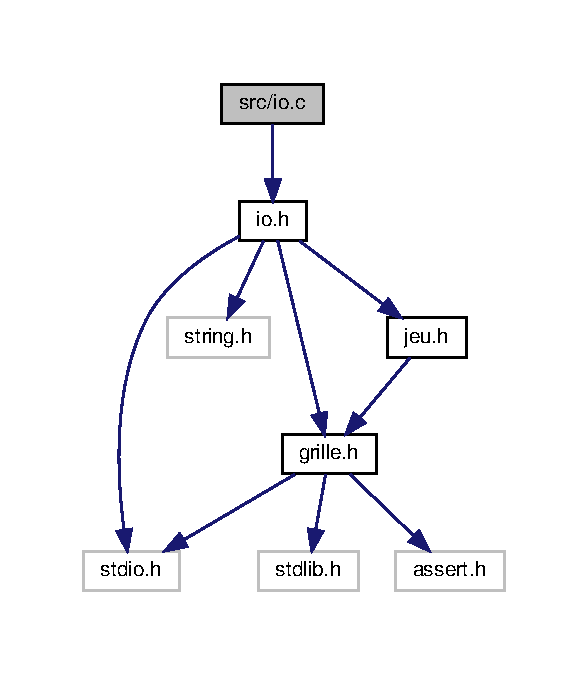
\includegraphics[width=282pt]{io_8c__incl}
\end{center}
\end{figure}
\subsection*{Fonctions}
\begin{DoxyCompactItemize}
\item 
void \hyperlink{io_8c_a634cf584c380ce221d5d4199f3e813bd}{affiche\+\_\+trait} (int c)
\begin{DoxyCompactList}\small\item\em Fonction d\textquotesingle{}affichage d\textquotesingle{}un trait horizontal. \end{DoxyCompactList}\item 
void \hyperlink{io_8c_a3f3ff78e56fcf21a932ff73b70635554}{affiche\+\_\+ligne} (int c, int $\ast$ligne)
\begin{DoxyCompactList}\small\item\em Fonction d\textquotesingle{}affichage d\textquotesingle{}une ligne de la grille. \end{DoxyCompactList}\item 
void \hyperlink{io_8c_a90cb8ec05374b46d9995705ed4954f34}{affiche\+\_\+grille} (\hyperlink{structgrille}{grille} g)
\begin{DoxyCompactList}\small\item\em Fonction d\textquotesingle{}affichage d\textquotesingle{}une grille. \end{DoxyCompactList}\item 
void \hyperlink{io_8c_ab36a6f8957cd3e682119007836ce6ad5}{efface\+\_\+grille} (\hyperlink{structgrille}{grille} g)
\begin{DoxyCompactList}\small\item\em Fonction d\textquotesingle{}effacement d\textquotesingle{}une grille. \end{DoxyCompactList}\item 
void \hyperlink{io_8c_a88493b3c55828670e47150a95ed7db5b}{debut\+\_\+jeu} (\hyperlink{structgrille}{grille} $\ast$g, \hyperlink{structgrille}{grille} $\ast$gc)
\begin{DoxyCompactList}\small\item\em Fonction pour débuter le jeu. Saisir la touche q permet de quitter le jeu, entrée permet de faire évoluer le jeu d\textquotesingle{}un temps, n permet d\textquotesingle{}entrée une nouvelle grille (ex \+: grille1). \end{DoxyCompactList}\end{DoxyCompactItemize}


\subsection{Description détaillée}
Gestion des entrées/sorties du jeu de la vie. 

\begin{DoxyAuthor}{Auteur}
Massimo Venuti 
\end{DoxyAuthor}
\begin{DoxyVersion}{Version}
1.\+0
\end{DoxyVersion}
Affichage des grilles et gestion des saisies du joueur lors du jeu de la vie. 

\subsection{Documentation des fonctions}
\mbox{\Hypertarget{io_8c_a90cb8ec05374b46d9995705ed4954f34}\label{io_8c_a90cb8ec05374b46d9995705ed4954f34}} 
\index{io.\+c@{io.\+c}!affiche\+\_\+grille@{affiche\+\_\+grille}}
\index{affiche\+\_\+grille@{affiche\+\_\+grille}!io.\+c@{io.\+c}}
\subsubsection{\texorpdfstring{affiche\+\_\+grille()}{affiche\_grille()}}
{\footnotesize\ttfamily void affiche\+\_\+grille (\begin{DoxyParamCaption}\item[{\hyperlink{structgrille}{grille}}]{g }\end{DoxyParamCaption})}



Fonction d\textquotesingle{}affichage d\textquotesingle{}une grille. 


\begin{DoxyParams}{Paramètres}
{\em g} & Grille \+: grille à afficher. \\
\hline
\end{DoxyParams}
\mbox{\Hypertarget{io_8c_a3f3ff78e56fcf21a932ff73b70635554}\label{io_8c_a3f3ff78e56fcf21a932ff73b70635554}} 
\index{io.\+c@{io.\+c}!affiche\+\_\+ligne@{affiche\+\_\+ligne}}
\index{affiche\+\_\+ligne@{affiche\+\_\+ligne}!io.\+c@{io.\+c}}
\subsubsection{\texorpdfstring{affiche\+\_\+ligne()}{affiche\_ligne()}}
{\footnotesize\ttfamily void affiche\+\_\+ligne (\begin{DoxyParamCaption}\item[{int}]{c,  }\item[{int $\ast$}]{ligne }\end{DoxyParamCaption})}



Fonction d\textquotesingle{}affichage d\textquotesingle{}une ligne de la grille. 


\begin{DoxyParams}{Paramètres}
{\em c} & Entier \+: nombre de colonnes de la grille. \\
\hline
{\em ligne} & Tableau d\textquotesingle{}entiers \+: ligne de la grille. \\
\hline
\end{DoxyParams}
\mbox{\Hypertarget{io_8c_a634cf584c380ce221d5d4199f3e813bd}\label{io_8c_a634cf584c380ce221d5d4199f3e813bd}} 
\index{io.\+c@{io.\+c}!affiche\+\_\+trait@{affiche\+\_\+trait}}
\index{affiche\+\_\+trait@{affiche\+\_\+trait}!io.\+c@{io.\+c}}
\subsubsection{\texorpdfstring{affiche\+\_\+trait()}{affiche\_trait()}}
{\footnotesize\ttfamily void affiche\+\_\+trait (\begin{DoxyParamCaption}\item[{int}]{c }\end{DoxyParamCaption})}



Fonction d\textquotesingle{}affichage d\textquotesingle{}un trait horizontal. 


\begin{DoxyParams}{Paramètres}
{\em c} & Entier \+: nombre de colonnes de la grille. \\
\hline
\end{DoxyParams}
\mbox{\Hypertarget{io_8c_a88493b3c55828670e47150a95ed7db5b}\label{io_8c_a88493b3c55828670e47150a95ed7db5b}} 
\index{io.\+c@{io.\+c}!debut\+\_\+jeu@{debut\+\_\+jeu}}
\index{debut\+\_\+jeu@{debut\+\_\+jeu}!io.\+c@{io.\+c}}
\subsubsection{\texorpdfstring{debut\+\_\+jeu()}{debut\_jeu()}}
{\footnotesize\ttfamily void debut\+\_\+jeu (\begin{DoxyParamCaption}\item[{\hyperlink{structgrille}{grille} $\ast$}]{g,  }\item[{\hyperlink{structgrille}{grille} $\ast$}]{gc }\end{DoxyParamCaption})}



Fonction pour débuter le jeu. Saisir la touche q permet de quitter le jeu, entrée permet de faire évoluer le jeu d\textquotesingle{}un temps, n permet d\textquotesingle{}entrée une nouvelle grille (ex \+: grille1). 


\begin{DoxyParams}{Paramètres}
{\em gc} & Adresse de la grille servant de copie temporaire pour le programme. \\
\hline
{\em g} & Adresse de la grille en jeu. \\
\hline
\end{DoxyParams}
\mbox{\Hypertarget{io_8c_ab36a6f8957cd3e682119007836ce6ad5}\label{io_8c_ab36a6f8957cd3e682119007836ce6ad5}} 
\index{io.\+c@{io.\+c}!efface\+\_\+grille@{efface\+\_\+grille}}
\index{efface\+\_\+grille@{efface\+\_\+grille}!io.\+c@{io.\+c}}
\subsubsection{\texorpdfstring{efface\+\_\+grille()}{efface\_grille()}}
{\footnotesize\ttfamily void efface\+\_\+grille (\begin{DoxyParamCaption}\item[{\hyperlink{structgrille}{grille}}]{g }\end{DoxyParamCaption})}



Fonction d\textquotesingle{}effacement d\textquotesingle{}une grille. 


\begin{DoxyParams}{Paramètres}
{\em g} & Grille \+: grille à effacer. \\
\hline
\end{DoxyParams}

\hypertarget{jeu_8c}{}\section{Référence du fichier src/jeu.c}
\label{jeu_8c}\index{src/jeu.\+c@{src/jeu.\+c}}


Evolutions du jeu de la vie.  


{\ttfamily \#include \char`\"{}jeu.\+h\char`\"{}}\newline
Graphe des dépendances par inclusion de jeu.\+c\+:
\nopagebreak
\begin{figure}[H]
\begin{center}
\leavevmode
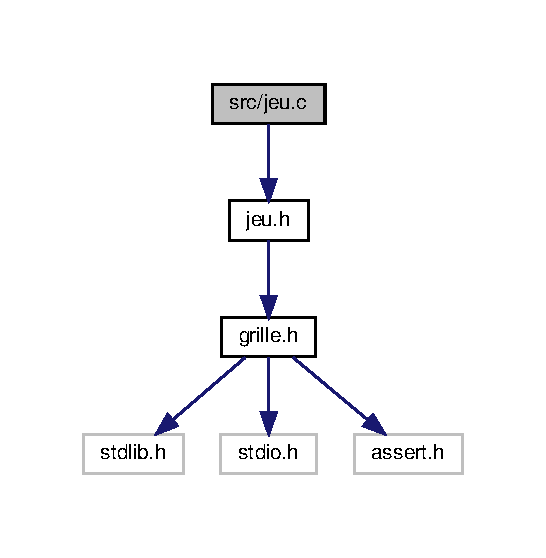
\includegraphics[width=262pt]{jeu_8c__incl}
\end{center}
\end{figure}
\subsection*{Fonctions}
\begin{DoxyCompactItemize}
\item 
int \hyperlink{jeu_8c_a919a35926d94b71717909ecc50233f26}{compte\+\_\+voisins\+\_\+vivants\+\_\+cyclique} (int i, int j, \hyperlink{structgrille}{grille} g)
\begin{DoxyCompactList}\small\item\em Fonction renvoyant le nombre de voisins vivants d\textquotesingle{}une cellule \mbox{[}i,j\mbox{]} -\/ les bords sont cycliques. \end{DoxyCompactList}\item 
int \hyperlink{jeu_8c_a2e8fdd206d197391527920bbbc137eef}{compte\+\_\+voisins\+\_\+vivants\+\_\+non\+\_\+cyclique} (int i, int j, \hyperlink{structgrille}{grille} g)
\begin{DoxyCompactList}\small\item\em Fonction renvoyant le nombre de voisins vivants d\textquotesingle{}une cellule \mbox{[}i,j\mbox{]} -\/ les bords ne sont pas cycliques. \end{DoxyCompactList}\item 
\mbox{\Hypertarget{jeu_8c_a35492cdc239f17e2ef5fd447c11db14a}\label{jeu_8c_a35492cdc239f17e2ef5fd447c11db14a}} 
void \hyperlink{jeu_8c_a35492cdc239f17e2ef5fd447c11db14a}{toggle\+\_\+compte\+\_\+voisins\+\_\+vivants} ()
\begin{DoxyCompactList}\small\item\em Fonction activant/désactivant le mode cyclique. \end{DoxyCompactList}\item 
\mbox{\Hypertarget{jeu_8c_af5dc5f87c713e0c76ead7327db4518f0}\label{jeu_8c_af5dc5f87c713e0c76ead7327db4518f0}} 
void \hyperlink{jeu_8c_af5dc5f87c713e0c76ead7327db4518f0}{toggle\+\_\+vieillissement} ()
\begin{DoxyCompactList}\small\item\em Fonction activant/désactivant le vieillissement. \end{DoxyCompactList}\item 
int \hyperlink{jeu_8c_a97d70fd6528087d6d64f63510f62b65d}{periode\+\_\+oscillation\+\_\+courante} (\hyperlink{structgrille}{grille} g)
\begin{DoxyCompactList}\small\item\em Fonction renvoyant la période d\textquotesingle{}oscillation d\textquotesingle{}une grille dans son état courant. \end{DoxyCompactList}\item 
int \hyperlink{jeu_8c_aba0c5411f74b76f13ccb2eac63175753}{periode\+\_\+oscillation\+\_\+delai} (\hyperlink{structgrille}{grille} g)
\begin{DoxyCompactList}\small\item\em Fonction renvoyant la période d\textquotesingle{}oscillation d\textquotesingle{}une grille en considérant un éventuel délai. \end{DoxyCompactList}\item 
void \hyperlink{jeu_8c_ada8f751a97ad1847db23c5ba17be7802}{evolue} (\hyperlink{structgrille}{grille} $\ast$g, \hyperlink{structgrille}{grille} $\ast$gc)
\begin{DoxyCompactList}\small\item\em Fonction faisant évoluer une grille d\textquotesingle{}un pas de temps. \end{DoxyCompactList}\end{DoxyCompactItemize}
\subsection*{Variables}
\begin{DoxyCompactItemize}
\item 
\mbox{\Hypertarget{jeu_8c_af587b56ea61a80b468caff5a89715cd7}\label{jeu_8c_af587b56ea61a80b468caff5a89715cd7}} 
int($\ast$ \hyperlink{jeu_8c_af587b56ea61a80b468caff5a89715cd7}{compte\+\_\+voisins\+\_\+vivants} )(int, int, \hyperlink{structgrille}{grille}) = \&\hyperlink{jeu_8h_a919a35926d94b71717909ecc50233f26}{compte\+\_\+voisins\+\_\+vivants\+\_\+cyclique}
\begin{DoxyCompactList}\small\item\em Pointeur de fonction contenant l\textquotesingle{}adresse de la fonction de calcul du voisinage d\textquotesingle{}une cellule. \end{DoxyCompactList}\item 
\mbox{\Hypertarget{jeu_8c_a852233e3ec97f7c44944c67998337e26}\label{jeu_8c_a852233e3ec97f7c44944c67998337e26}} 
int \hyperlink{jeu_8c_a852233e3ec97f7c44944c67998337e26}{vieillissement} = V\+I\+E\+I\+L\+L\+I\+S\+S\+E\+M\+E\+N\+T\+\_\+\+I\+N\+IT
\begin{DoxyCompactList}\small\item\em Valeur contenant 1 ou 0 selon si le vieillissement des cellules est activé ou non. \end{DoxyCompactList}\end{DoxyCompactItemize}


\subsection{Description détaillée}
Evolutions du jeu de la vie. 

\begin{DoxyAuthor}{Auteur}
Massimo Venuti 
\end{DoxyAuthor}


\subsection{Documentation des fonctions}
\mbox{\Hypertarget{jeu_8c_a919a35926d94b71717909ecc50233f26}\label{jeu_8c_a919a35926d94b71717909ecc50233f26}} 
\index{jeu.\+c@{jeu.\+c}!compte\+\_\+voisins\+\_\+vivants\+\_\+cyclique@{compte\+\_\+voisins\+\_\+vivants\+\_\+cyclique}}
\index{compte\+\_\+voisins\+\_\+vivants\+\_\+cyclique@{compte\+\_\+voisins\+\_\+vivants\+\_\+cyclique}!jeu.\+c@{jeu.\+c}}
\subsubsection{\texorpdfstring{compte\+\_\+voisins\+\_\+vivants\+\_\+cyclique()}{compte\_voisins\_vivants\_cyclique()}}
{\footnotesize\ttfamily int compte\+\_\+voisins\+\_\+vivants\+\_\+cyclique (\begin{DoxyParamCaption}\item[{int}]{i,  }\item[{int}]{j,  }\item[{\hyperlink{structgrille}{grille}}]{g }\end{DoxyParamCaption})}



Fonction renvoyant le nombre de voisins vivants d\textquotesingle{}une cellule \mbox{[}i,j\mbox{]} -\/ les bords sont cycliques. 


\begin{DoxyParams}{Paramètres}
{\em i} & Entier \+: i-\/ème ligne de la grille. \\
\hline
{\em j} & Entier \+: j-\/ème colonne de la grille. \\
\hline
{\em g} & Grille \+: grille en jeu. \\
\hline
\end{DoxyParams}
\begin{DoxyReturn}{Renvoie}
Entier \+: nombre de voisins vivants de la cellule. 
\end{DoxyReturn}
\mbox{\Hypertarget{jeu_8c_a2e8fdd206d197391527920bbbc137eef}\label{jeu_8c_a2e8fdd206d197391527920bbbc137eef}} 
\index{jeu.\+c@{jeu.\+c}!compte\+\_\+voisins\+\_\+vivants\+\_\+non\+\_\+cyclique@{compte\+\_\+voisins\+\_\+vivants\+\_\+non\+\_\+cyclique}}
\index{compte\+\_\+voisins\+\_\+vivants\+\_\+non\+\_\+cyclique@{compte\+\_\+voisins\+\_\+vivants\+\_\+non\+\_\+cyclique}!jeu.\+c@{jeu.\+c}}
\subsubsection{\texorpdfstring{compte\+\_\+voisins\+\_\+vivants\+\_\+non\+\_\+cyclique()}{compte\_voisins\_vivants\_non\_cyclique()}}
{\footnotesize\ttfamily int compte\+\_\+voisins\+\_\+vivants\+\_\+non\+\_\+cyclique (\begin{DoxyParamCaption}\item[{int}]{i,  }\item[{int}]{j,  }\item[{\hyperlink{structgrille}{grille}}]{g }\end{DoxyParamCaption})}



Fonction renvoyant le nombre de voisins vivants d\textquotesingle{}une cellule \mbox{[}i,j\mbox{]} -\/ les bords ne sont pas cycliques. 


\begin{DoxyParams}{Paramètres}
{\em i} & Entier \+: i-\/ème ligne de la grille. \\
\hline
{\em j} & Entier \+: j-\/ème colonne de la grille. \\
\hline
{\em g} & Grille \+: grille en jeu. \\
\hline
\end{DoxyParams}
\begin{DoxyReturn}{Renvoie}
Entier \+: nombre de voisins vivants de la cellule. 
\end{DoxyReturn}
\mbox{\Hypertarget{jeu_8c_ada8f751a97ad1847db23c5ba17be7802}\label{jeu_8c_ada8f751a97ad1847db23c5ba17be7802}} 
\index{jeu.\+c@{jeu.\+c}!evolue@{evolue}}
\index{evolue@{evolue}!jeu.\+c@{jeu.\+c}}
\subsubsection{\texorpdfstring{evolue()}{evolue()}}
{\footnotesize\ttfamily void evolue (\begin{DoxyParamCaption}\item[{\hyperlink{structgrille}{grille} $\ast$}]{g,  }\item[{\hyperlink{structgrille}{grille} $\ast$}]{gc }\end{DoxyParamCaption})}



Fonction faisant évoluer une grille d\textquotesingle{}un pas de temps. 


\begin{DoxyParams}{Paramètres}
{\em gc} & Adresse de la grille servant de copie temporaire pour le programme. \\
\hline
{\em g} & Adresse de la grille en jeu. \\
\hline
\end{DoxyParams}
\mbox{\Hypertarget{jeu_8c_a97d70fd6528087d6d64f63510f62b65d}\label{jeu_8c_a97d70fd6528087d6d64f63510f62b65d}} 
\index{jeu.\+c@{jeu.\+c}!periode\+\_\+oscillation\+\_\+courante@{periode\+\_\+oscillation\+\_\+courante}}
\index{periode\+\_\+oscillation\+\_\+courante@{periode\+\_\+oscillation\+\_\+courante}!jeu.\+c@{jeu.\+c}}
\subsubsection{\texorpdfstring{periode\+\_\+oscillation\+\_\+courante()}{periode\_oscillation\_courante()}}
{\footnotesize\ttfamily int periode\+\_\+oscillation\+\_\+courante (\begin{DoxyParamCaption}\item[{\hyperlink{structgrille}{grille}}]{g }\end{DoxyParamCaption})}



Fonction renvoyant la période d\textquotesingle{}oscillation d\textquotesingle{}une grille dans son état courant. 


\begin{DoxyParams}{Paramètres}
{\em g} & Grille \+: grille en jeu. \\
\hline
\end{DoxyParams}
\begin{DoxyReturn}{Renvoie}
Entier \+: période d\textquotesingle{}oscillation, 0 si elle n\textquotesingle{}existe pas. 
\end{DoxyReturn}
\mbox{\Hypertarget{jeu_8c_aba0c5411f74b76f13ccb2eac63175753}\label{jeu_8c_aba0c5411f74b76f13ccb2eac63175753}} 
\index{jeu.\+c@{jeu.\+c}!periode\+\_\+oscillation\+\_\+delai@{periode\+\_\+oscillation\+\_\+delai}}
\index{periode\+\_\+oscillation\+\_\+delai@{periode\+\_\+oscillation\+\_\+delai}!jeu.\+c@{jeu.\+c}}
\subsubsection{\texorpdfstring{periode\+\_\+oscillation\+\_\+delai()}{periode\_oscillation\_delai()}}
{\footnotesize\ttfamily int periode\+\_\+oscillation\+\_\+delai (\begin{DoxyParamCaption}\item[{\hyperlink{structgrille}{grille}}]{g }\end{DoxyParamCaption})}



Fonction renvoyant la période d\textquotesingle{}oscillation d\textquotesingle{}une grille en considérant un éventuel délai. 


\begin{DoxyParams}{Paramètres}
{\em g} & Grille \+: grille en jeu. \\
\hline
\end{DoxyParams}
\begin{DoxyReturn}{Renvoie}
Entier \+: période d\textquotesingle{}oscillation, 0 si elle n\textquotesingle{}existe pas. 
\end{DoxyReturn}

\hypertarget{main_8c}{}\section{Référence du fichier src/main.c}
\label{main_8c}\index{src/main.\+c@{src/main.\+c}}


Jeu de la vie.  


{\ttfamily \#include $<$stdio.\+h$>$}\newline
{\ttfamily \#include \char`\"{}grille.\+h\char`\"{}}\newline
{\ttfamily \#include \char`\"{}io.\+h\char`\"{}}\newline
{\ttfamily \#include \char`\"{}jeu.\+h\char`\"{}}\newline
Graphe des dépendances par inclusion de main.\+c\+:\nopagebreak
\begin{figure}[H]
\begin{center}
\leavevmode
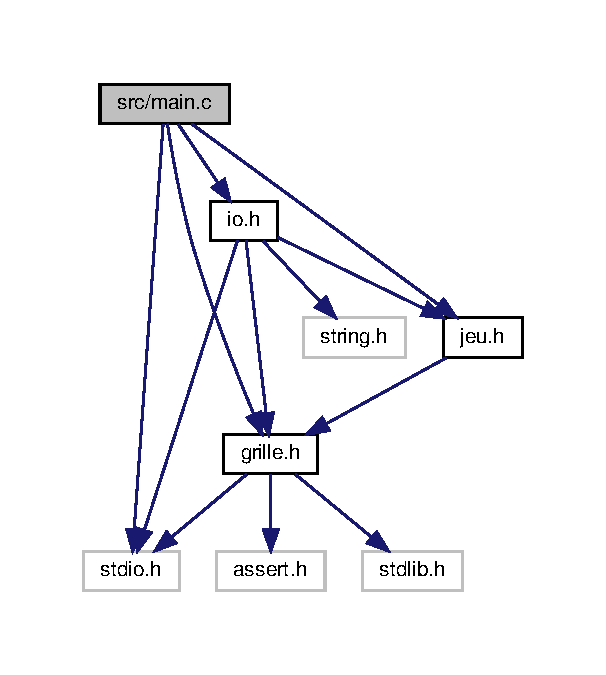
\includegraphics[width=291pt]{main_8c__incl}
\end{center}
\end{figure}
\subsection*{Fonctions}
\begin{DoxyCompactItemize}
\item 
int \hyperlink{main_8c_a3c04138a5bfe5d72780bb7e82a18e627}{main} (int argc, char $\ast$$\ast$argv)
\begin{DoxyCompactList}\small\item\em Entrée du programme. \end{DoxyCompactList}\end{DoxyCompactItemize}


\subsection{Description détaillée}
Jeu de la vie. 

\begin{DoxyAuthor}{Auteur}
Massimo Venuti
\end{DoxyAuthor}
Programme de base du jeu de la vie mettant en scène une série de grilles initiales prédéfinies pouvant être séléctionnées par le joueur. 

\subsection{Documentation des fonctions}
\mbox{\Hypertarget{main_8c_a3c04138a5bfe5d72780bb7e82a18e627}\label{main_8c_a3c04138a5bfe5d72780bb7e82a18e627}} 
\index{main.\+c@{main.\+c}!main@{main}}
\index{main@{main}!main.\+c@{main.\+c}}
\subsubsection{\texorpdfstring{main()}{main()}}
{\footnotesize\ttfamily int main (\begin{DoxyParamCaption}\item[{int}]{argc,  }\item[{char $\ast$$\ast$}]{argv }\end{DoxyParamCaption})}



Entrée du programme. 


\begin{DoxyParams}{Paramètres}
{\em argc} & Chaine de caractères \+: nom du programme. \\
\hline
{\em argv} & Chaine de caractères \+: nom de la grille à charger. \\
\hline
\end{DoxyParams}
\begin{DoxyReturn}{Renvoie}
0 si aucune erreur. 
\end{DoxyReturn}

%--- End generated contents ---

% Index
\backmatter
\newpage
\phantomsection
\clearemptydoublepage
\addcontentsline{toc}{chapter}{Index}
\printindex

\end{document}
